\documentclass{standalone}

\usepackage{tikz}
\usepackage{standalone}
\usepackage{color}
\usetikzlibrary{matrix}
\usetikzlibrary{shapes.geometric}
\usetikzlibrary{shapes.misc}

\begin{document}

	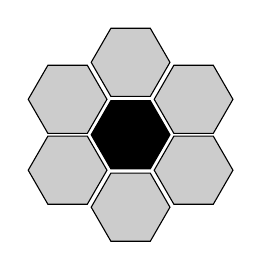
\begin{tikzpicture}
	
	\tikzstyle{cell}=[regular polygon,regular polygon sides=6, draw=black, minimum size=1cm];

	\node[fill=black] at (0, 0) [cell] {};
	\node[fill=black!20] at (.8, 0.45) [cell] {};
	\node[fill=black!20] at (.8, -0.45) [cell] {};
	\node[fill=black!20] at (-.8, 0.45) [cell] {};
	\node[fill=black!20] at (-.8, -0.45) [cell] {};
	\node[fill=black!20] at (0, -.92) [cell] {};
	\node[fill=black!20] at (0, 0.92) [cell] {};

	\end{tikzpicture}

\end{document}
